\documentclass{article}

\usepackage{graphicx}
\usepackage{tikz}
\usepackage{tikzsymbols}
\usetikzlibrary{calc,patterns,shapes.geometric}
\pagestyle{empty}
\usepackage[margin=0pt]{geometry}
\geometry{papersize={14in,12in}}

\def\centerarc[#1](#2)(#3:#4:#5){\draw[#1] ($(#2)+({#5*cos(#3)},{#5*sin(#3)})$) arc (#3:#4:#5);}

\begin{document}
	\begin{figure}
		\centering
		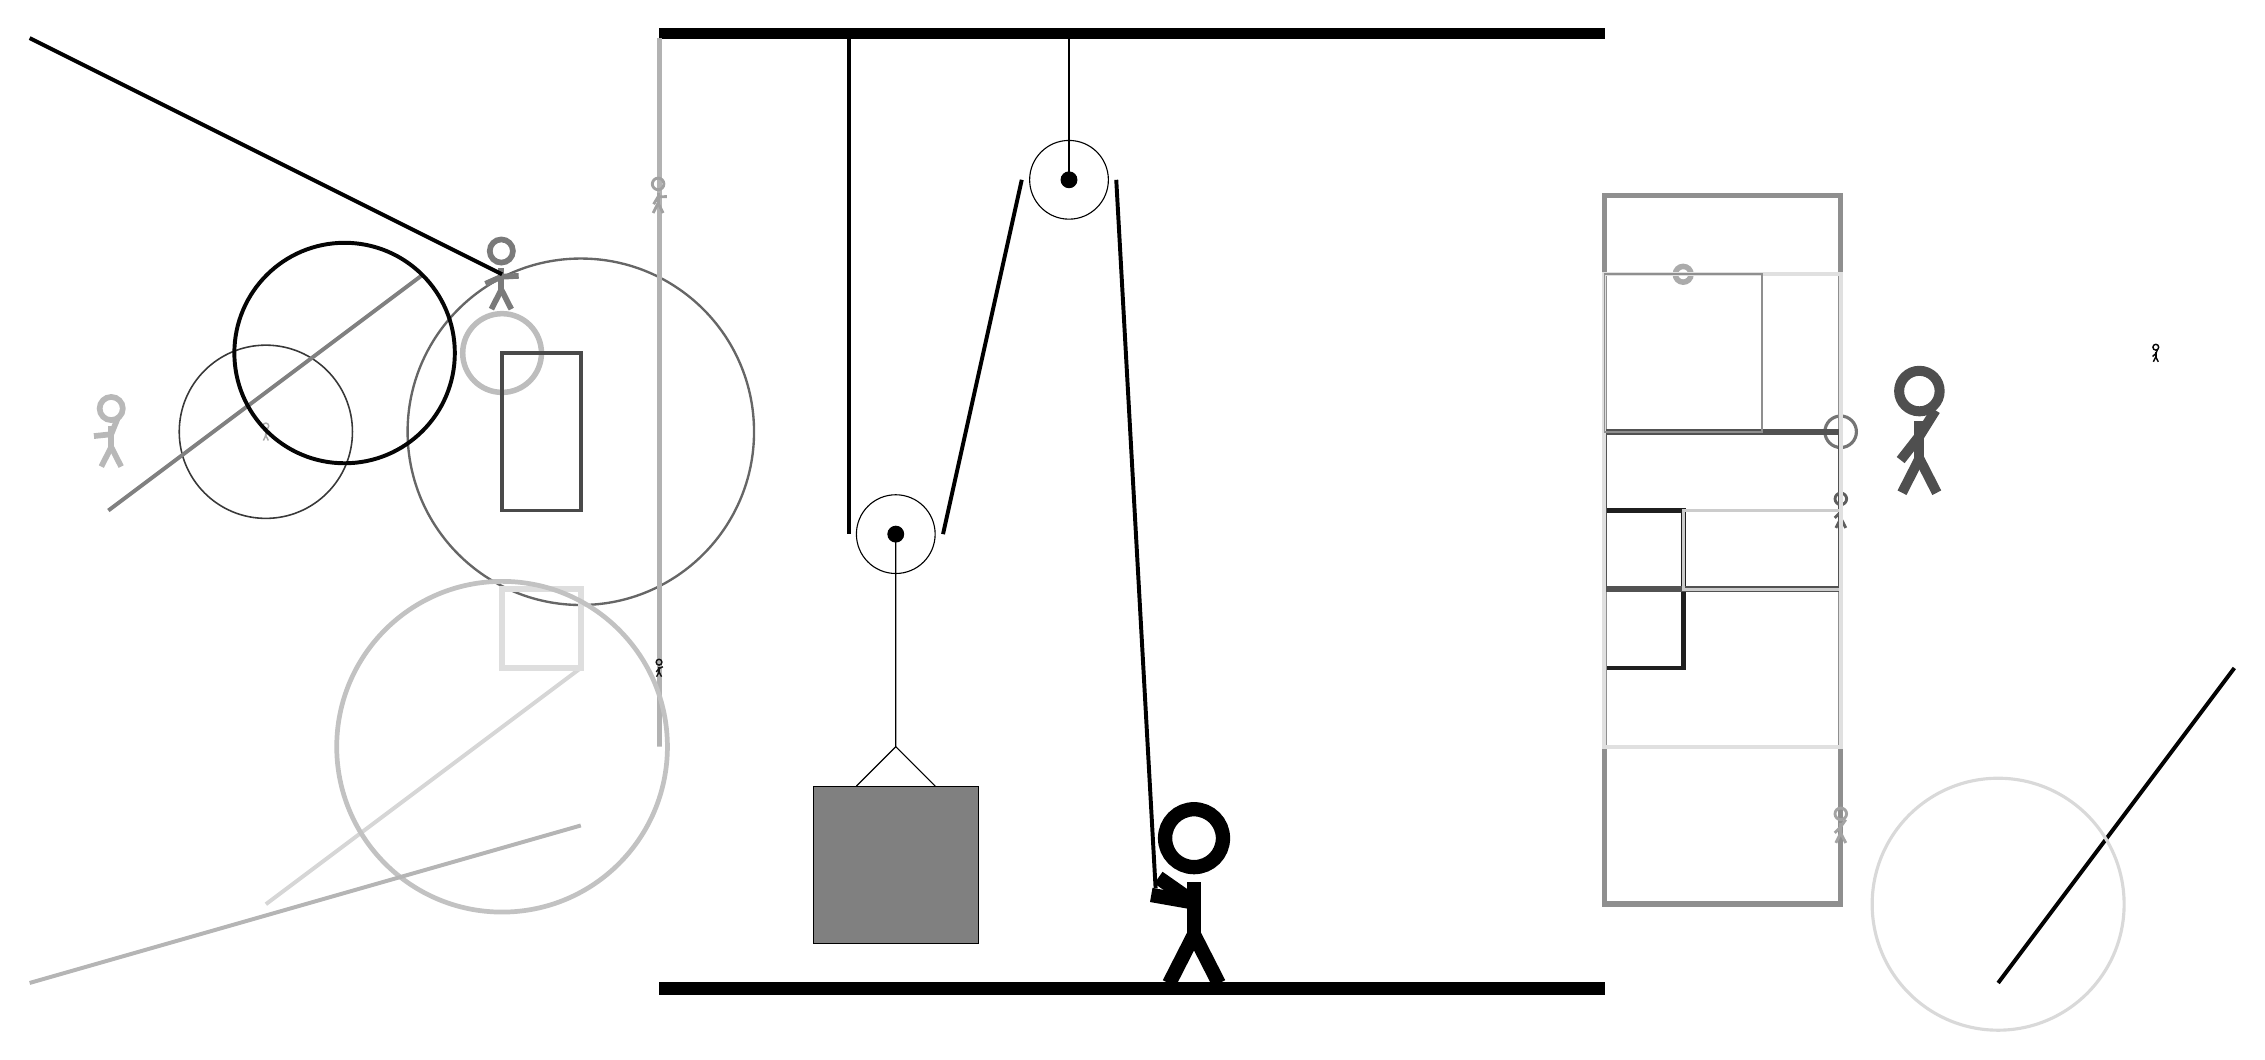
\begin{tikzpicture}
			%%%%% START %%%%%
			
			\draw[fill=black] (-2, 9) rectangle (10, 9.125);
			
			\draw (3.2, 7.2) circle (0.5);
			\draw[fill=black] (3.2, 7.2) circle (0.1);
			\draw[thick] (3.2, 7.2) -- (3.2, 9);
			
			\draw (1, 2.7) circle (0.5);
			\draw[fill=black] (1, 2.7) circle (0.1);
			
			\draw (1, 2.7) -- (1, 0) -- (0.5, -0.5);
			\draw (1, 0) -- (1.5, -0.5);
			\draw[fill=black!50] (-0.05, -0.5) rectangle (2.05, -2.5);
			
			\draw[line width=0.5mm] (0.4, 9) -- (0.4, 2.7);
			\centerarc[line width=0.5mm](1, 2.7)(180:360:0.6);
			\draw[line width=0.5mm](1.6, 2.7) -- (2.6, 7.2);
			\centerarc[line width=0.5mm](3.2, 7.2)(0:180:0.6);
			\draw[line width=0.5mm](3.8, 7.2) -- (4.3, -1.8);
			
			\node at (4.7, -1.9) {\Strichmaxerl[10][-35][170]};
			
			\draw [line width=0.3mm, color=black!60](-3, 4) circle (2.2);
			
			\draw [line width=0.7mm, color=black!26](-4, 5) circle (0.5);
			\draw[line width=0.6mm, color=black!88] (11, 3) rectangle (10, 1);
			\node[line width=0.2mm, color=black!69] at (14, 4) {\Strichmaxerl[7][52][58]};
			
			\node[line width=0.5mm, color=black!33] at (-7, 4) {\Strichmaxerl[1][83][62]};
			
			\draw [line width=0.7mm, color=black!33](11, 6) circle (0.1);
			\draw[line width=0.5mm, color=black!16](-7, -2) -- (-3, 1);
			
			\draw[line width=0.5mm, color=black!99](15, -3) -- (18, 1);
			\draw[line width=0.7mm, color=black!13] (-4, 2) rectangle (-3, 1);
			
			\draw[line width=0.7mm, color=black!30] (-2, 9) rectangle (-2, 0);
			
			\draw [line width=0.4mm, color=black!54](13, 4) circle (0.2);
			
			\node[line width=0.3mm, color=black!98] at (17, 5) {\Strichmaxerl[1][41][68]};
			\draw [line width=0.2mm, color=black!78](-7, 4) circle (1.1);
			\draw [line width=0.6mm, color=black!24](-4, 0) circle (2.1);
			\node[line width=0.2mm, color=black!52] at (-4, 6) {\Strichmaxerl[4][24][3]};
			\draw[line width=0.5mm, color=black!29](-3, -1) -- (-10, -3);
			
			\draw[line width=0.7mm, color=black!44] (10, 7) rectangle (13, -2);
			\draw[line width=0.7mm, color=black!68] (10, 2) rectangle (13, 4);
			\node[line width=0.3mm, color=black!63] at (13, 3) {\Strichmaxerl[2][45][90]};
			
			\node[line width=0.3mm, color=black!36] at (13, -1) {\Strichmaxerl[2][46][55]};
			\draw[line width=0.5mm, color=black!50](-5, 6) -- (-9, 3);
			\draw[line width=0.5mm, color=black!100](-4, 6) -- (-10, 9);
			\draw[line width=0.4mm, color=black!20] (11, 3) rectangle (13, 2);
			\node[line width=0.4mm, color=black!28] at (-9, 4) {\Strichmaxerl[4][6][68]};
			\draw[line width=0.5mm, color=black!71] (-3, 3) rectangle (-4, 5);
			
			\draw[line width=0.5mm, color=black!12] (10, 0) rectangle (13, 6);
			\draw [line width=0.5mm, color=black!98](-6, 5) circle (1.4);
			\node[line width=0.7mm, color=black!92] at (-2, 1) {\Strichmaxerl[1][49][26]};
			\node[line width=0.5mm, color=black!37] at (-2, 7) {\Strichmaxerl[2][59][1]};
			\draw[line width=0.2mm, color=black!44] (12, 4) rectangle (10, 6);
			\draw [line width=0.4mm, color=black!15](15, -2) circle (1.6);
			
			\draw[fill=black] (-2, -3) rectangle (10, -3.15);
			
			%%%%% END %%%%%
		\end{tikzpicture}
	\end{figure}	
\end{document}